%%%% Paramétrage du TD %%%%
\def\xxnumchapitre{Chapitre 1 \vspace{.2cm}}
\def\xxchapitre{\hspace{.12cm} Découverte de l'algorithmique et de la programmation}

\def\xxcompetences{%
\textsl{%
\textbf{Savoirs et compétences :}\\
\vspace{-.4cm}
\begin{itemize}[label=\ding{112},font=\color{bleuxp}] 
\item .
%\item \textit{Mod3.C2 : } pôles dominants et réduction de l’ordre du modèle : principe, justification
%\item \textit{Res2.C4 : } stabilité des SLCI : définition entrée bornée -- sortie bornée (EB -- SB)	
%\item \textit{Res2.C5 : } stabilité des SLCI : équation caractéristique	
%\item \textit{Res2.C6 : } stabilité des SLCI : position des pôles dans le plan complexe
%\item \textit{Res2.C7 : } stabilité des SLCI : marges de stabilité (de gain et de phase)
\end{itemize}
}}


\def\xxfigures{
%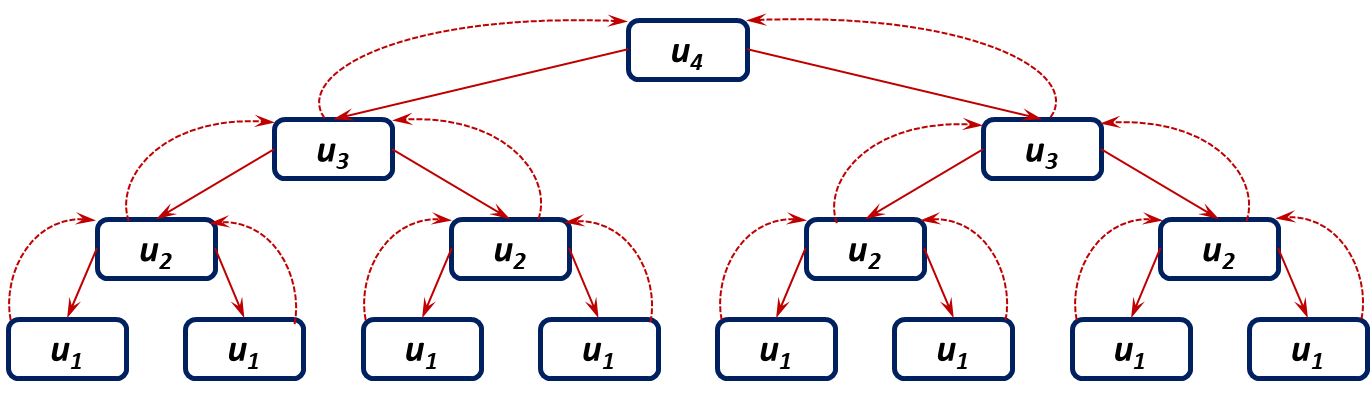
\includegraphics[width=3cm]{fig_01}\\
%\textit{}
}%figues de la page de garde

\def\xxtitreexo{QCM 01}
\def\xxsourceexo{}
\def\xxactivite{{QCM 01} \ifprof  -- Corrigé \else \fi}

%\iflivret
\input{\repRel/Style/pagegarde_TD}
%\else
%\pagestyle{empty}


%%%%%%%% PAGE DE GARDE COURS
\ifcours
\begin{tikzpicture}[remember picture,overlay]
\node at (current page.north west)
{\begin{tikzpicture}[remember picture,overlay]
\node[anchor=north west,inner sep=0pt] at (0,0) {\includegraphics[width=\paperwidth]{\thechapterimage}};
\draw[anchor=west] (-2cm,-8cm) node [line width=2pt,rounded corners=15pt,draw=ocre,fill=white,fill opacity=0.6,inner sep=40pt]{\strut\makebox[22cm]{}};
\draw[anchor=west] (1cm,-8cm) node {\huge\sffamily\bfseries\color{black} %
\begin{minipage}{1cm}
\rotatebox{90}{\LARGE\sffamily\textsc{\color{ocre}\textbf{\xxnumpartie}}}
\end{minipage} \hfill
\begin{minipage}[c]{14cm}
\begin{titrepartie}
\begin{flushright}
\renewcommand{\baselinestretch}{1.1} 
\Large\sffamily\textsc{\textbf{\xxpartie}}
\renewcommand{\baselinestretch}{1} 
\end{flushright}
\end{titrepartie}
\end{minipage} \hfill
\begin{minipage}[c]{3.5cm}
{\large\sffamily\textsc{\textbf{\color{ocre} \discipline}}}
\end{minipage} 
 };
\end{tikzpicture}};
\end{tikzpicture}


\begin{tikzpicture}[overlay]
\node[shape=rectangle, 
      rounded corners = .25 cm,
	  draw= ocre,
	  line width=2pt, 
	  fill = ocre!10,
	  minimum width  = 2.5cm,
	  minimum height = 3cm,] at (18cm,0) {};
\node at (17.7cm,0) {\rotatebox{90}{\textbf{\Large\color{ocre}{\classe}}}};
%{};
\end{tikzpicture}

\vspace{3.5cm}

\begin{tikzpicture}[remember picture,overlay]
\draw[anchor=west] (-2cm,-6cm) node {\huge\sffamily\bfseries\color{black} %
\begin{minipage}{2cm}
\begin{center}
\LARGE\sffamily\textsc{\color{ocre}\textbf{\xxactivite}}
\end{center}
\end{minipage} \hfill
\begin{minipage}[c]{15cm}
\begin{titrechapitre}
\renewcommand{\baselinestretch}{1.1} 
\Large\sffamily\textsc{\textbf{\xxnumchapitre}}

\Large\sffamily\textsc{\textbf{\xxchapitre}}
\vspace{.5cm}

\renewcommand{\baselinestretch}{1} 
\normalsize\normalfont
\xxcompetences
\end{titrechapitre}
\end{minipage}  };
\end{tikzpicture}
\vfill

\begin{flushright}
\begin{minipage}[c]{.3\linewidth}
\begin{center}
\xxfigures
\end{center}
\end{minipage}\hfill
\begin{minipage}[c]{.6\linewidth}
\startcontents
\printcontents{}{1}{}
\end{minipage}
\end{flushright}

\begin{tikzpicture}[remember picture,overlay]
\draw[anchor=west] (4.5cm,-.7cm) node {
\begin{minipage}[c]{.2\linewidth}
\begin{flushright}

\includegraphics[width=2cm]{png/logoCC}
\end{flushright}
\end{minipage}
\begin{minipage}[c]{.2\linewidth}
\textsl{\xxauteur} \\
\textsl{\classe}
\end{minipage}
 };
\end{tikzpicture}
\newpage
\pagestyle{fancy}

\newpage
\pagestyle{fancy}

\else
\fi


%%%%%%%% PAGE DE GARDE TD
\iftd
%\begin{tikzpicture}[remember picture,overlay]
%\node at (current page.north west)
%{\begin{tikzpicture}[remember picture,overlay]
%\draw[anchor=west] (-2cm,-3.25cm) node [line width=2pt,rounded corners=15pt,draw=ocre,fill=white,fill opacity=0.6,inner sep=40pt]{\strut\makebox[22cm]{}};
%\draw[anchor=west] (1cm,-3.25cm) node {\huge\sffamily\bfseries\color{black} %
%\begin{minipage}{1cm}
%\rotatebox{90}{\LARGE\sffamily\textsc{\color{ocre}\textbf{\xxnumpartie}}}
%\end{minipage} \hfill
%\begin{minipage}[c]{13.5cm}
%\begin{titrepartie}
%\begin{flushright}
%\renewcommand{\baselinestretch}{1.1} 
%\Large\sffamily\textsc{\textbf{\xxpartie}}
%\renewcommand{\baselinestretch}{1} 
%\end{flushright}
%\end{titrepartie}
%\end{minipage} \hfill
%\begin{minipage}[c]{3.5cm}
%{\large\sffamily\textsc{\textbf{\color{ocre} \discipline}}}
%\end{minipage} 
% };
%\end{tikzpicture}};
%\end{tikzpicture}

%%%%%%%%%% PAGE DE GARDE TD %%%%%%%%%%%%%%%
%\begin{tikzpicture}[overlay]
%\node[shape=rectangle, 
%      rounded corners = .25 cm,
%	  draw= ocre,
%	  line width=2pt, 
%	  fill = ocre!10,
%	  minimum width  = 2.5cm,
%	  minimum height = 2.5cm,] at (18.5cm,0) {};
%\node at (17.7cm,0) {\rotatebox{90}{\textbf{\Large\color{ocre}{\classe}}}};
%%{};
%\end{tikzpicture}

% PARTIE ET CHAPITRE
%\begin{tikzpicture}[remember picture,overlay]
%\draw[anchor=west] (-1cm,-2.1cm) node {\large\sffamily\bfseries\color{black} %
%\begin{minipage}[c]{15cm}
%\begin{flushleft}
%\xxnumchapitre \\
%\xxchapitre
%\end{flushleft}
%\end{minipage}  };
%\end{tikzpicture}

% Bandeau titre exo
\begin{tikzpicture}[remember picture,overlay]
\draw[anchor=west] (-2cm,-4cm) node {\huge\sffamily\bfseries\color{black} %
\begin{minipage}{5cm}
\begin{center}
\LARGE\sffamily\color{ocre}\textbf{\textsc{\xxactivite}}

\begin{center}
\xxfigures
\end{center}

\end{center}
\end{minipage} \hfill
\begin{minipage}[c]{12cm}
\begin{titrechapitre}
\renewcommand{\baselinestretch}{1.1} 
\large\sffamily\textbf{\textsc{\xxtitreexo}}

\small\sffamily{\textbf{\textit{\color{black!70}\xxsourceexo}}}
\vspace{.5cm}

\renewcommand{\baselinestretch}{1} 
\normalsize\normalfont
\xxcompetences
\end{titrechapitre}
\end{minipage}  };
\end{tikzpicture}
\else
\fi


%%%%%%%% PAGE DE GARDE FICHE
\iffiche
\begin{tikzpicture}[remember picture,overlay]
\node at (current page.north west)
{\begin{tikzpicture}[remember picture,overlay]
\draw[anchor=west] (-2cm,-3.25cm) node [line width=2pt,rounded corners=15pt,draw=ocre,fill=white,fill opacity=0.6,inner sep=40pt]{\strut\makebox[22cm]{}};
\draw[anchor=west] (1cm,-3.25cm) node {\huge\sffamily\bfseries\color{black} %
\begin{minipage}{1cm}
\rotatebox{90}{\LARGE\sffamily\textsc{\color{ocre}\textbf{\xxnumpartie}}}
\end{minipage} \hfill
\begin{minipage}[c]{14cm}
\begin{titrepartie}
\begin{flushright}
\renewcommand{\baselinestretch}{1.1} 
\large\sffamily\textsc{\textbf{\xxpartie} \\} 

\vspace{.2cm}

\normalsize\sffamily\textsc{\textbf{\xxnumchapitre -- \xxchapitre}}
\renewcommand{\baselinestretch}{1} 
\end{flushright}
\end{titrepartie}
\end{minipage} \hfill
\begin{minipage}[c]{3.5cm}
{\large\sffamily\textsc{\textbf{\color{ocre} \discipline}}}
\end{minipage} 
 };
\end{tikzpicture}};
\end{tikzpicture}


\begin{tikzpicture}[overlay]
\node[shape=rectangle, 
      rounded corners = .25 cm,
	  draw= ocre,
	  line width=2pt, 
	  fill = ocre!10,
	  minimum width  = 2.5cm,
	  minimum height = 2.5cm,] at (18.5cm,0.5cm) {};
%	  minimum height = 2.5cm,] at (18.5cm,0cm) {};
\node at (17.7cm,0.5) {\rotatebox{90}{\textsf{\textbf{\large\color{ocre}{\classe}}}}};
%{};
\end{tikzpicture}

\else
\fi



%\fi

\setlength{\columnseprule}{.1pt}

\pagestyle{fancy}
\thispagestyle{plain}

\vspace{4.5cm}

\def\columnseprulecolor{\color{bleuxp}}
\setlength{\columnseprule}{0.4pt} 

%%%%%%%%%%%%%%%%%%%%%%%




\ifprof
\vspace{1cm}
\else
\begin{multicols}{2}
\fi

\subsection*{Types de variables}
\subsubsection*{Choix de type}

\question{Quel type choisiriez-vous pour représenter les données suivantes ?}
Vous justifierez brièvement chaque réponse. 

\begin{enumerate}[label = \emph{\alph*)}]
  \item Le nom d'une personne.
  \item L'état civil d'une personne : nom, prénom, date de naissance, nationalité.
  \item Les coordonnées d'un point dans l'espace.
  \item L'historique du nombre de $5/2$ dans la classe de MP du lycée. 
  \item Un numéro de téléphone. 
  \item \emph{Plus difficile :} l'arbre généalogique de vos ancêtres. 
\end{enumerate}


\question{Dans chaque cas, indiquez le type que vous utiliseriez pour modéliser les grandeurs suivantes dans leur contexte scientifique usuel.
Vous justifierez brièvement chaque réponse. }

\begin{enumerate}[label=\emph{\alph*)}]
  \item La taille d'un individu en mètres. 
  \item Le tour de taille d'un manequin, en millimètres.
  \item Le nombre d'Avogadro.
  \item Le nombre de Joules dans une calorie.
  \item Le nombre de secondes dans une année.
  \item Le plus grand nombre premier représentable avec 20 chiffres en écriture binaire.
\end{enumerate}

\subsubsection*{Booléens}
\setcounter{numques}{0}

\question{Déterminer la valeur des expressions suivantes.}

\begin{multicols}{2}
  \begin{enumerate}[label=\emph{\alph*)}]
    \item \texttt{0 == 42}
    \item \texttt{1 = 1}
    \item \texttt{3 == 3.}
    \item \texttt{0 != 1}
    \item \texttt{0 < 1}
    \item \texttt{4. >= 4}
    \item \texttt{0 !< 1}
    \item \texttt{2*True + False}
    \item \texttt{-1 <= True}
    \item \texttt{1 == True}
    \item \texttt{False != 0.}
    \item \texttt{True and False}
    \item \texttt{True or False}
    \item \texttt{True or True}
    \item \texttt{(2 == 3-1) or (1/0 == 5)}
    \item \texttt{(1/0 == 5) or (2 == 3-1)}
    \item \texttt{(True or True) and False}
    \item \texttt{True or (True and False)}
    \item \texttt{(False or True) and False}    
    \item \texttt{False or (True and False)}    
    \item \texttt{not (1 == 1 or 4 == 5)}
    \item \texttt{(not 1 == 1) or 4 == 5}
    \item \texttt{(not True) or True}
  \end{enumerate}
\end{multicols}

\subsubsection*{Chaînes de caractères}

\question{Prévoir les résultats des expressions suivantes, puis le vérifier grâce à l'interpréteur interactif.}

\begin{multicols}{2}
  \begin{enumerate}[label=\emph{\alph*)}]
    \item \texttt{"abba"}
    \item \texttt{abba}
    \item \texttt{""}
    \item \texttt{"" == " "}
    \item \texttt{""+""}
    \item \texttt{""+"" == ""}
    \item \texttt{"May"+" "+"04th"}
    \item \texttt{"12"+3}
    \item \texttt{"12"+"trois"}
    \item \texttt{len("abracadabra")}
    \item \texttt{len("")}
    \item \texttt{len("lamartin"+"2015")}
  \end{enumerate}
\end{multicols}

\question{Pour chaque séquence d'instruction, prévoir son résultat puis le vérifier grâce à l'interpréteur interactif.}

\begin{enumerate}[label=\emph{\alph*)}]
\item 
\begin{lstlisting}
t = "oh oui youpi !"
print(t)
t[0]
t[-1]
t[1]
t[2]
t[1] = "o" 
\end{lstlisting}
\end{enumerate}

\begin{enumerate}[label=\emph{\alph*)}]
\setcounter{enumi}{1}
\item
\begin{lstlisting}
ex = "abdefgh"
"a" in ex
a in ex
"def" in ex
"adf" in ex
\end{lstlisting}
\end{enumerate}


\subsubsection*{$n-$uplés}
\question{Prévoir les résultats des expressions suivantes.}

\begin{multicols}{2}
  \begin{enumerate}[label=\emph{\alph*)}]
%    \item \texttt{(1,2)}
%    \item \texttt{(1)}
%    \item \texttt{(1,)}
%    \item \texttt{(,)}
%    \item \texttt{()}
%    \item \texttt{()+()}
%    \item \texttt{()+() == ()}
    \item \texttt{(1,2)+3}
    \item \texttt{(1,2)+(3)}
    \item \texttt{(1,2)+(3,)}
    \item \texttt{(1,2)+(3,4,5)}
    \item \texttt{len((1,7,2,"zzz",[]))}
    \item \texttt{len(())}
    \item \texttt{len(("a","bc")+("cde",""))}
  \end{enumerate}
\end{multicols}


\question{Pour chaque séquence d'instruction, prévoir son résultat.}

\begin{enumerate}[label=\emph{\alph*)}]
\item 
\begin{lstlisting}
t = (2,"abra",9,6*9,22)
print(t)
t[0]
t[-1]
t[1]
t[1] = "cadabra" 
\end{lstlisting}
\end{enumerate}

\begin{enumerate}[label=\emph{\alph*)}]
\setcounter{enumi}{1}
\item 
\begin{lstlisting}
res = (45,5)
x,y = res
(x,y) == x,y
(x,y) == (x,y)
print x
print(y)
x,y = y,x
print(y)
\end{lstlisting}
\end{enumerate}

\question{Pour chaque séquence d'instruction, prévoir son résultat.}

\begin{enumerate}[label=\emph{\alph*)}]
\item 
\begin{lstlisting}
t = (2,"abra",9,6*9,22)
print(t)
t[0]
t[-1]
t[1]
t[1] = "cadabra" 
\end{lstlisting}
\end{enumerate}
\begin{enumerate}[label=\emph{\alph*)}]
\setcounter{enumi}{1}
\item 
\begin{lstlisting}
res = (45,5)
x,y = res
(x,y) == x,y
(x,y) == (x,y)
print x
print(y)
x,y = y,x
print(y)
\end{lstlisting}
\end{enumerate}
\begin{enumerate}[label=\emph{\alph*)}]
\setcounter{enumi}{2}
\item 
\begin{lstlisting}
v = 7
ex = (-1,5,2,"","abra",8,3,v)
5 in ex
abra in ex
(2 in ex) and ("abr" in ex)
v in ex
\end{lstlisting}
\end{enumerate}



\subsubsection*{Listes}

\question{Prévoir les résultats des expressions suivantes, puis le vérifier grâce à l'interpréteur interactif d'IDLE.}

\begin{multicols}{2}
  \begin{enumerate}[label=\emph{\alph*)}]
    \item \texttt{[1,2,3,"a"]}
    \item \texttt{123a}
    \item \texttt{[]}
    \item \texttt{[]+[]}
    \item \texttt{[]+[] == []}
    \item \texttt{[1,2] + [5,7,9]}
    \item \texttt{[0,0]+[0]}
    \item \texttt{len(["a","b"])}
    \item \texttt{len([])}
    \item \texttt{len([[]])}
    \item \texttt{len([[[]]])}
    \item \texttt{len([0,0]+[1])}
  \end{enumerate}
\end{multicols}

\question{Pour chaque séquence d'instruction, prévoir son résultat puis le vérifier grâce à l'interpréteur interactif d'IDLE.}

\begin{enumerate}[label=\emph{\alph*)}]
\item 
\begin{lstlisting}
t = [1,2,3,4,5,6]
u = ["a","b","c","d"]
print(t+u)
t[0]
t[-1]
z = t[3]
print(z)
t.append(7)
print(t)
\end{lstlisting}
\end{enumerate}
\begin{enumerate}[label=\emph{\alph*)}]
\setcounter{enumi}{2}
\item
\begin{lstlisting}
ex = ["sin","cos","tan","log","exp"]
"log" in ex
log in ex
"l" in ex
z = ex.pop()
print(z)
z in ex
print(ex)
\end{lstlisting}
\end{enumerate}
\begin{enumerate}[label=\emph{\alph*)}]
\setcounter{enumi}{3}
\item 
\begin{lstlisting}
  u = [1,2,3,4,5,6]
  L = u
  u = [1,2,3,42,5,6]
  print(L)
\end{lstlisting}
\end{enumerate}
\begin{enumerate}[label=\emph{\alph*)}]
\setcounter{enumi}{4}
\item
\begin{lstlisting}
  u = [1,2,3,4,5,6]
  L = u
  u[3] = 42
  print(L)
\end{lstlisting}
\end{enumerate}

\subsection*{Suite d'expressions}


\question{}
\begin{enumerate}[label = \emph{\alph*)}]
  \item Affecter à \texttt{v} la liste \texttt{[2,5,3,-1,7,2,1]}
  \item Affecter à \texttt{L} la liste vide.
  \item Vérifier le type des variables crées.
  \item Calculer la longueur de \texttt{v}, affectée à \texttt{n} et celle de \texttt{L}, affectée à \texttt{m}.
  \item Tester les expressions suivantes : \texttt{v[0]}, \texttt{v[2]}, \texttt{v[n]}, \texttt{v[n-1]}, \texttt{v[-1]} et \texttt{v[-2]}.
  \item Changer la valeur du quatrième élément de \texttt{v}.
  \item Que renvoie \texttt{v[1:3]} ? Remplacer dans \texttt{v} les trois derniers éléments par leurs carrés.
  \item Que fait \texttt{v[1] = [0,0,0]} ? Combien d'éléments y a-t-il alors dans \texttt{v} ?
\end{enumerate}

\question{Voici des affectations successives des variables $a$ et $b$. Dresser un tableau donnant les valeurs 
de $a$ et $b$ à chaque étape.}

\begin{lstlisting}
>>>  a = 1
>>>  b = 5
>>>  a = b-3 
>>>  b = 2*a 	
>>>  a = a
>>>  a = b	
\end{lstlisting}


\ifprof
\else
\end{multicols}
\fi

